\documentclass[12pt, a4paper]{article}
\usepackage[a4paper, includeheadfoot, mag=1000, left=2cm, right=1.5cm, top=1.5cm, bottom=1.5cm, headsep=0.8cm, footskip=0.8cm]{geometry}
% Fonts
\usepackage{fontspec, unicode-math}
\setmainfont[Ligatures=TeX]{CMU Serif}
\setmonofont{CMU Typewriter Text}
\usepackage[english, russian]{babel}
% Indent first paragraph
\usepackage{indentfirst}
\setlength{\parskip}{5pt}
% Diagrams
\usepackage{graphicx}
\usepackage{float}
% Page headings
\usepackage{fancyhdr}
\pagestyle{fancy}
\renewcommand{\headrulewidth}{0pt}
\setlength{\headheight}{16pt}
%\newfontfamily\namefont[Scale=1.2]{Gloria Hallelujah}
\fancyhead{}


\usepackage{listings}
\lstdefinestyle{lablisting}{
  basicstyle=\scriptsize\ttfamily,
  numbers=left,
  stepnumber=1,
  otherkeywords={EOF, O\_RDONLY, STDIN\_FILENO, STDOUT\_FILENO, STDERR\_FILENO},
  numbersep=10pt,
  showspaces=false,
  showstringspaces=false
}

\graphicspath{ {images/} }

\newcommand{\specialcell}[2][l]{%
  \begin{tabular}[#1]{@{}l@{}}#2\end{tabular}}

\begin{document}

% Title page
\begin{titlepage}
\begin{center}

\textsc{Национальный исследовательский университет ИТМО\\[4mm]
Факультет программной инженерии и компьютерной техники}
\vfill
\textbf{Учебно-исследовательская работа №1\\[4mm]
по дисципение Сети ЭВМ и телекоммуникации\\[16mm]
}
\begin{flushright}
Студент: Саржевский Иван
\\[2mm]Группа: P3302
\end{flushright}
\vfill
г. Санкт-Петербург\\[2mm]
2020 г.

\end{center}
\end{titlepage}

\section*{Цель}

Изучение методов логического и физического кодирования, используемых в цифровых
сетях передачи данных.

\section*{Задание}

Выполнить логическое и физическое кодирование исходного сообщения в соответствии
с заданными методами кодирования, провести сравнительный анализ рассматриваемых
методов кодирования, выбрать и обосновать наилучший метод для передачи исходного
сообщения.

\section*{Ход работы}
\subsection*{Формирование сообщения}

\begin{tabular}{ l l }
  \textit{Сообщение:} & \texttt{Саржевский И.А.} \\
  \textit{Hex-код:} & \texttt{D1 E0 F0 E6 E5 E2 F1 EA E8 E9 20 C8 2E C0 2E} \\
  \textit{Bin-код:} & \specialcell[l]{ 
    \texttt{11010001 11100000 11110000 11100110 11100101 11100010 11110001} \\
    \texttt{11101010 11101000 11101001 00100000 11001000 00101110 11000000} \\
    \texttt{00101110}
  }
\end{tabular}

\subsection*{Физическое кодирование}

\subsubsection*{Определение частот}

Возьмем за основу разложение бесконечного сигнала \texttt{1010101010}... в ряд
Фурье.

\begin{figure}[h]
  \begin{center}
    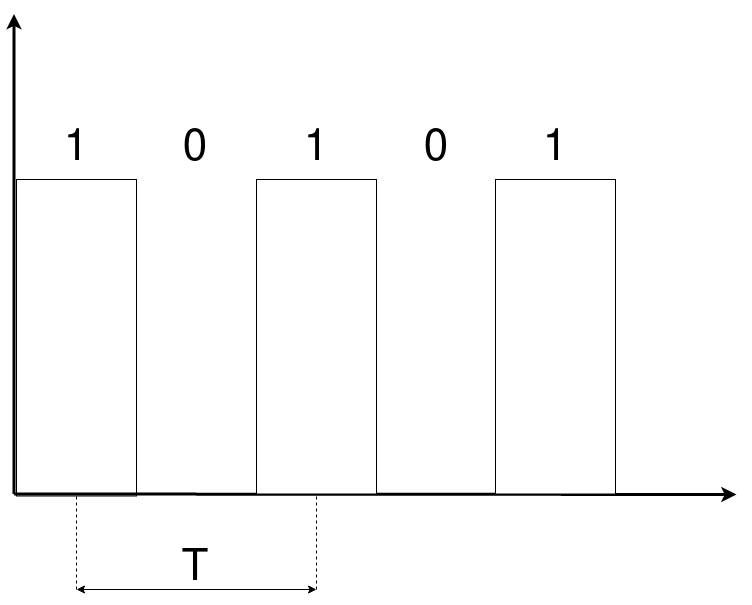
\includegraphics[scale=0.25]{one_zero}
    \caption{График сигнала бесконечного \texttt{10101010...}}
  \end{center}
\end{figure}

Его первые 4 гармоники:
$$A_0 \sin(2 \pi F_0 t) + (A_0 / 3) \sin(2 \pi 3 F_0 t) +
  (A_0 / 5) \sin(2 \pi 5 F_0 t) + (A_0 / 7) \sin(2 \pi 7 F_0 t)$$

\end{document}
